\documentclass[tikz]{standalone}
\usepackage{xcolor}

\definecolor{hse-hellblau}{cmyk}{.75,.1,.06,0}
\definecolor{hse-blau75}{HTML}{8abde2}
\definecolor{hse-blau50}{HTML}{b4d3ed}
\definecolor{hse-blau25}{HTML}{dbe9f7}
\definecolor{hse-blau15}{HTML}{eaf2fa}
\definecolor{hse-hellgrau}{cmyk}{0,0,0,.08}

\begin{document}
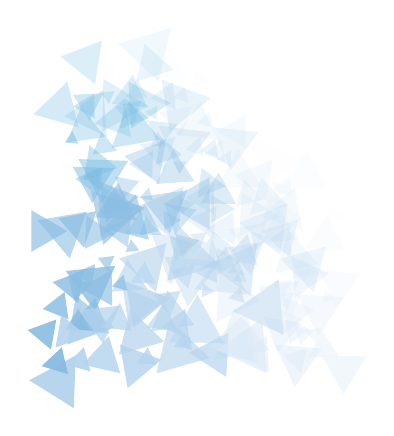
\begin{tikzpicture}

\foreach \n in {1,...,200} {
    \pgfmathsetmacro{\x}{random(0,100)}
    \pgfmathsetmacro{\y}{random(0,100)}
    \pgfmathsetmacro{\size}{random(5,20)}
    \pgfmathsetmacro{\rotation}{random(0,360)}
    
    % Farbauswahl basierend auf Position
    \pgfmathtruncatemacro{\colorIndex}{min(6, 1 + floor((\x+(100-\y))/50))}
    
    \pgfmathsetmacro{\opacity}{max(0, min(1, (150-\x-\y)/150))}
    
    \definecolor{selectedColor}{RGB}
    {\ifcase\colorIndex
        \or 119,189,226 % hse-hellblau
        \or 138,189,226 % hse-blau75
        \or 180,211,237 % hse-blau50
        \or 219,233,247 % hse-blau25
        \or 234,242,250 % hse-blau15
        \or 235,235,235 % hse-hellgrau
    \fi}
    
    \begin{scope}[shift={(\x pt, \y pt)}, rotate=\rotation]
        \pgfmathsetmacro{\height}{0.866*\size}
        \pgfmathsetmacro{\halfsize}{0.5*\size}
        \fill[selectedColor, opacity=\opacity] 
        (0,0) -- (\size pt,0) -- (\halfsize pt,\height pt) -- cycle;
    \end{scope}
}
\end{tikzpicture}
\end{document}